\appendix
\renewcommand*\appendixpagename{Anhang}
\appendixpage
\addcontentsline{toc}{chapter}{Anhang}
\renewcommand{\thefigure}{A.\arabic{figure}}

\chapter*{Messergebnisse}

\begin{figure}[tbh]
	\centering
		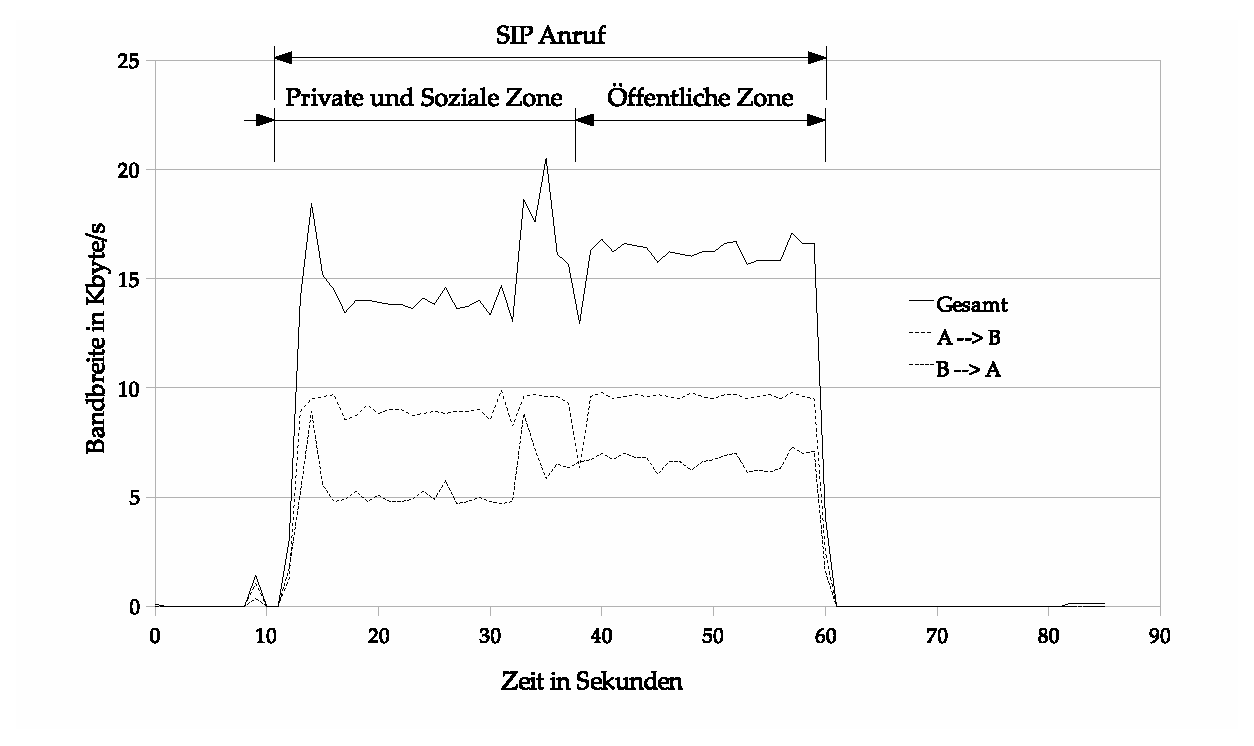
\includegraphics[width=.90\textwidth]{grafiken/ohnevadupdown.eps}
	\caption{Der Up- und Downstream ohne Unterscheidung der Zonen}
	\label{fig:NOVADrtpsip}
\end{figure}

\begin{figure}[tbh]
	\centering
		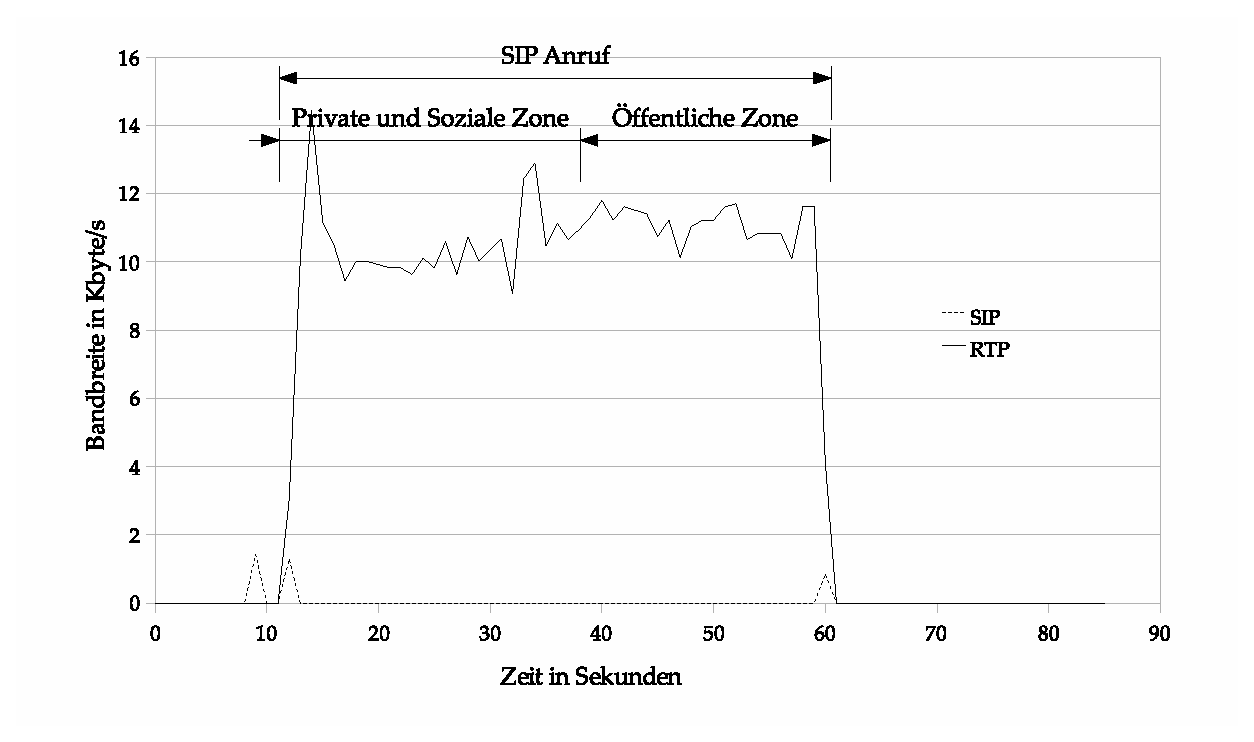
\includegraphics[width=.90\textwidth]{grafiken/ohnevadsiprtp.eps}
		\caption{Signalisierung mit SIP, Audiostrom mit RTP ohne Unterscheidung der Zonen}
	\label{fig:NoVADupdown}
\end{figure}

\begin{figure}[tbh]
	\centering
		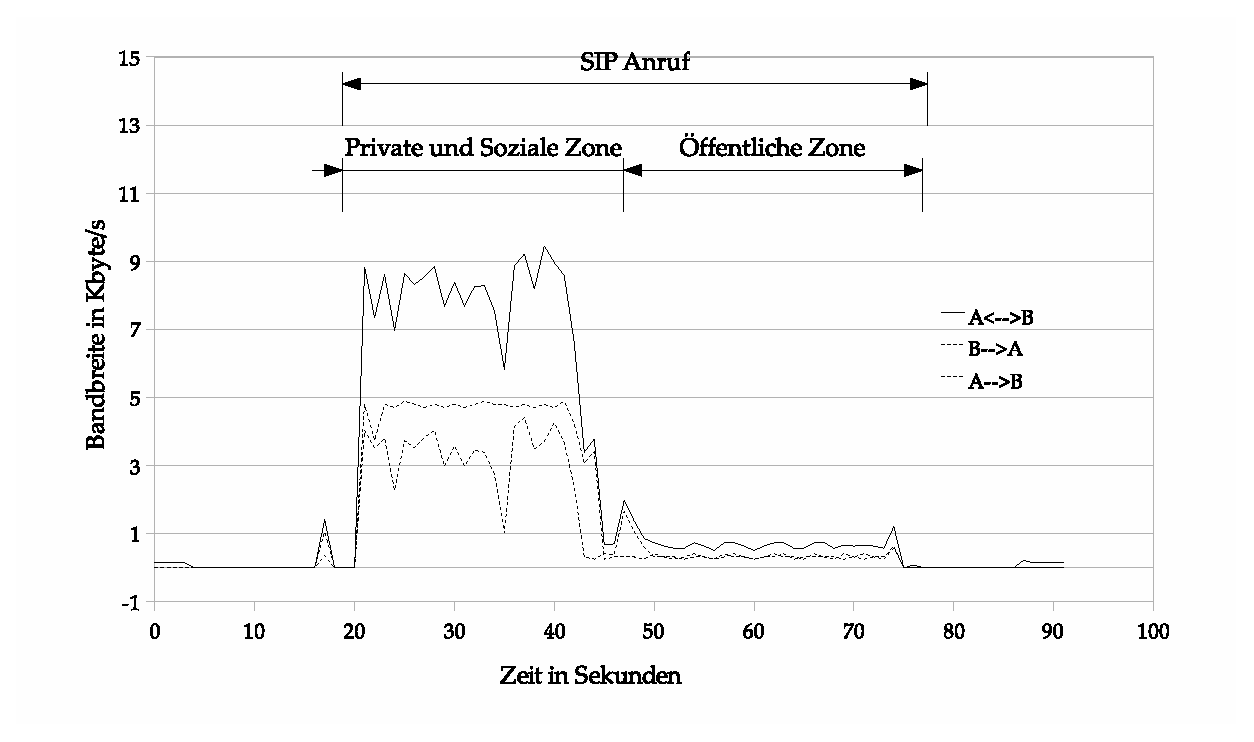
\includegraphics[width=1.00\textwidth]{grafiken/mitvadupdown.eps}
		\caption{Der Up- und Downstream mit der Silcence-Supression-Technik}
	\label{fig:VADupdown}
\end{figure}

\begin{figure}[tbh]
	\centering
		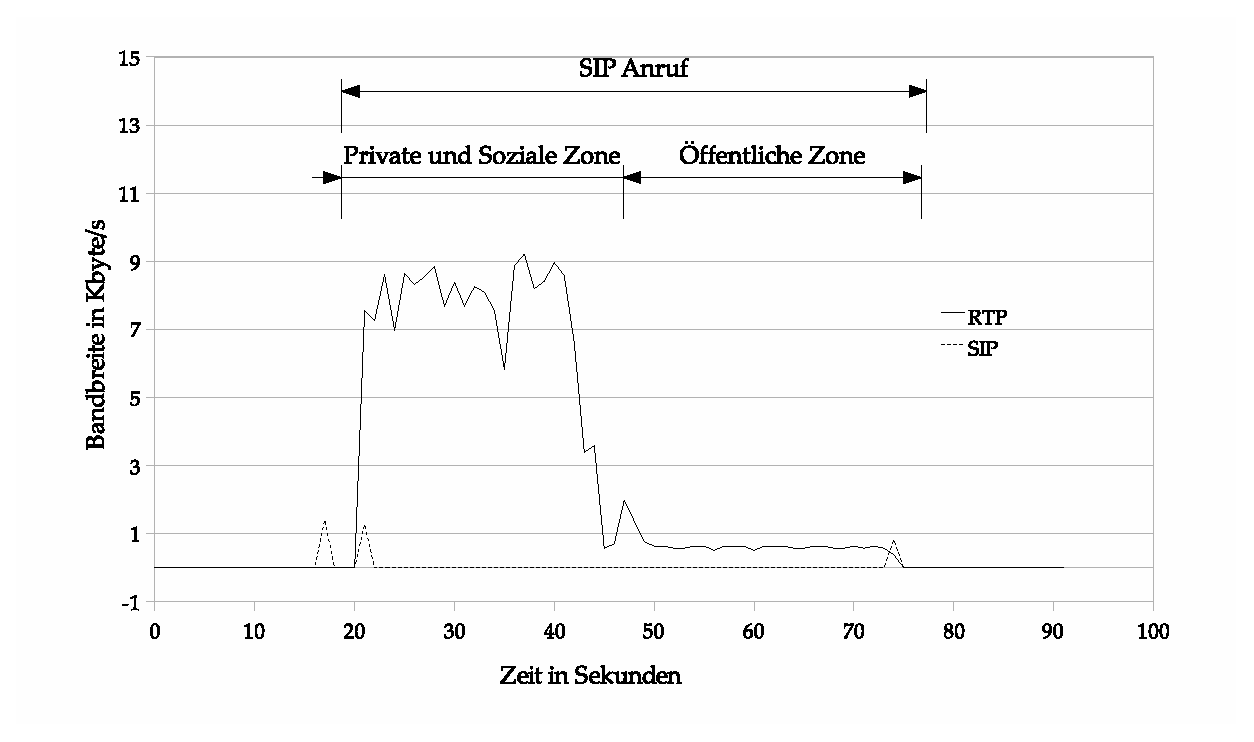
\includegraphics[width=1.00\textwidth]{grafiken/mitvadrtpsip.eps}
		\caption{Der Up- und Downstream mit der Silcence-Supression-Technik}
	\label{fig:VADrtpsip}
\end{figure}

\begin{figure}[tbh]
	\centering
		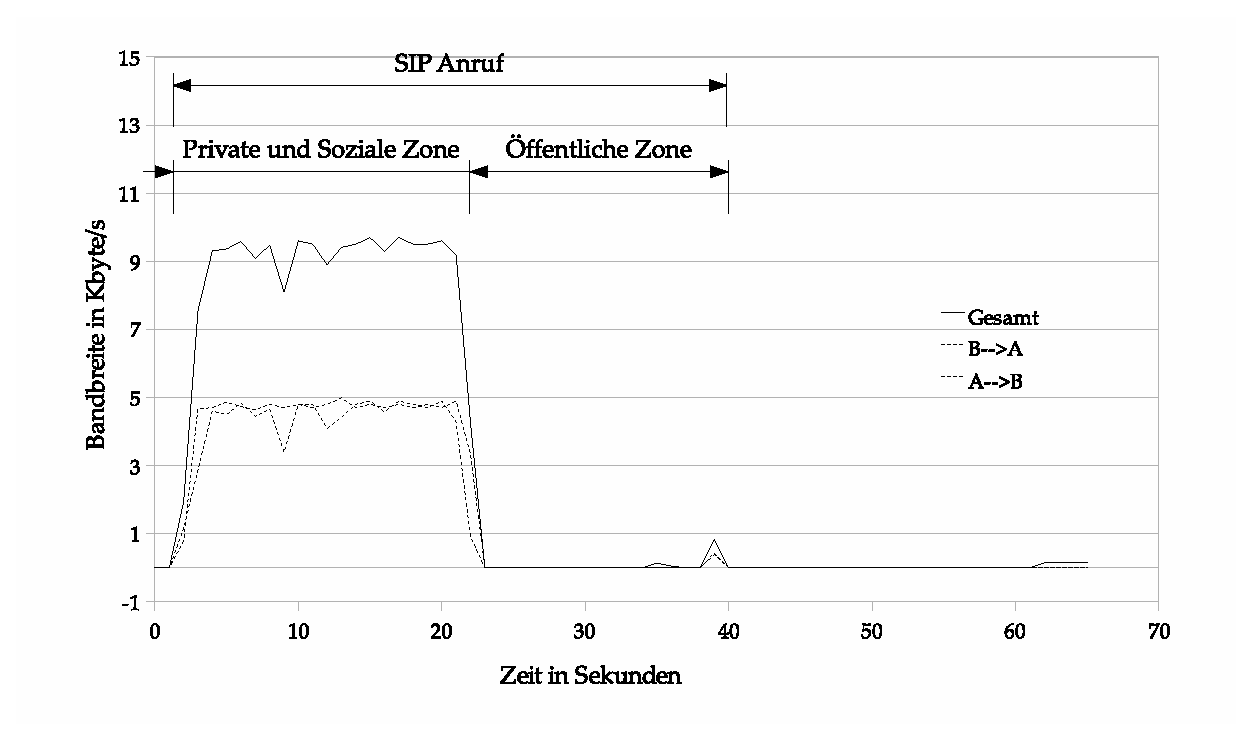
\includegraphics[width=1.00\textwidth]{grafiken/mitholdupanddown.eps}
		\caption{Der Up- und Downstream mit der SIP-Hold-Technik}
	\label{fig:mitholdupanddown}
\end{figure}

\begin{figure}[tbh]
	\centering
		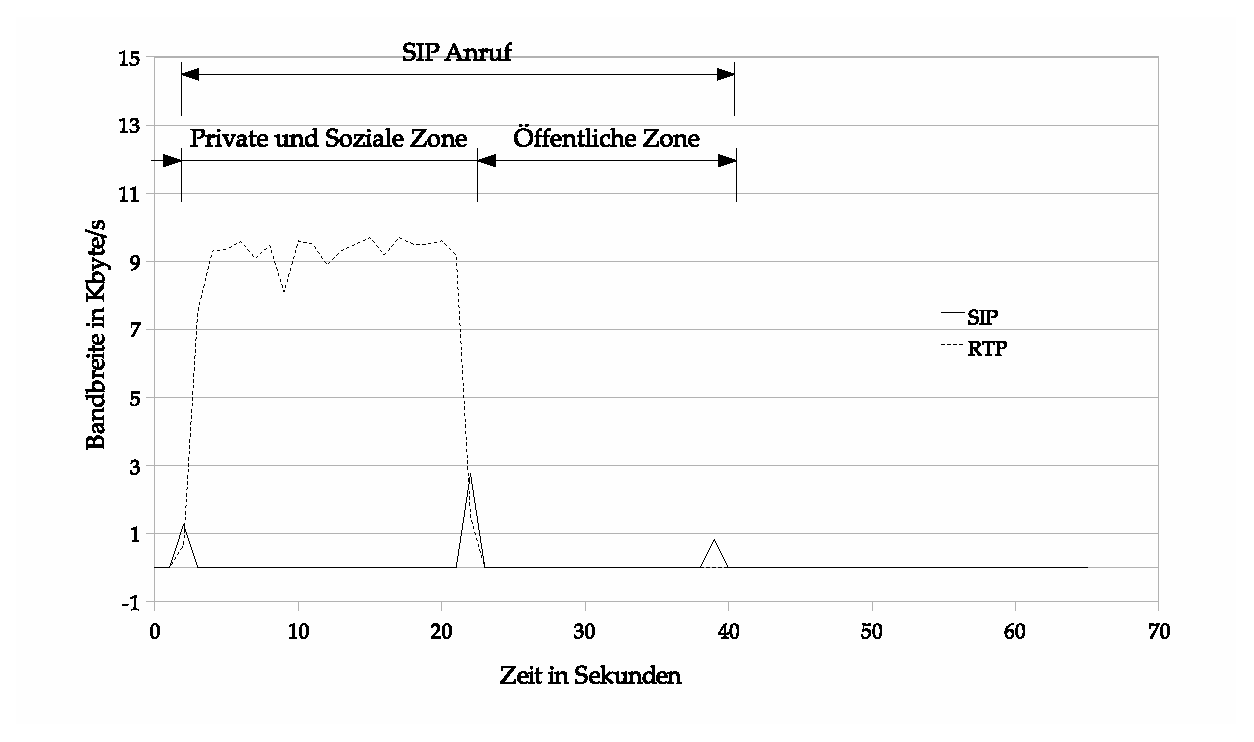
\includegraphics[width=1.00\textwidth]{grafiken/mithold1.eps}
		\caption{Gegen�berstellung des SIP- und RTP-Traffics mit der SIP-HOLD-Technik}
	\label{fig:mithold1}
\end{figure}


\begin{figure}[tbh]
	\centering
		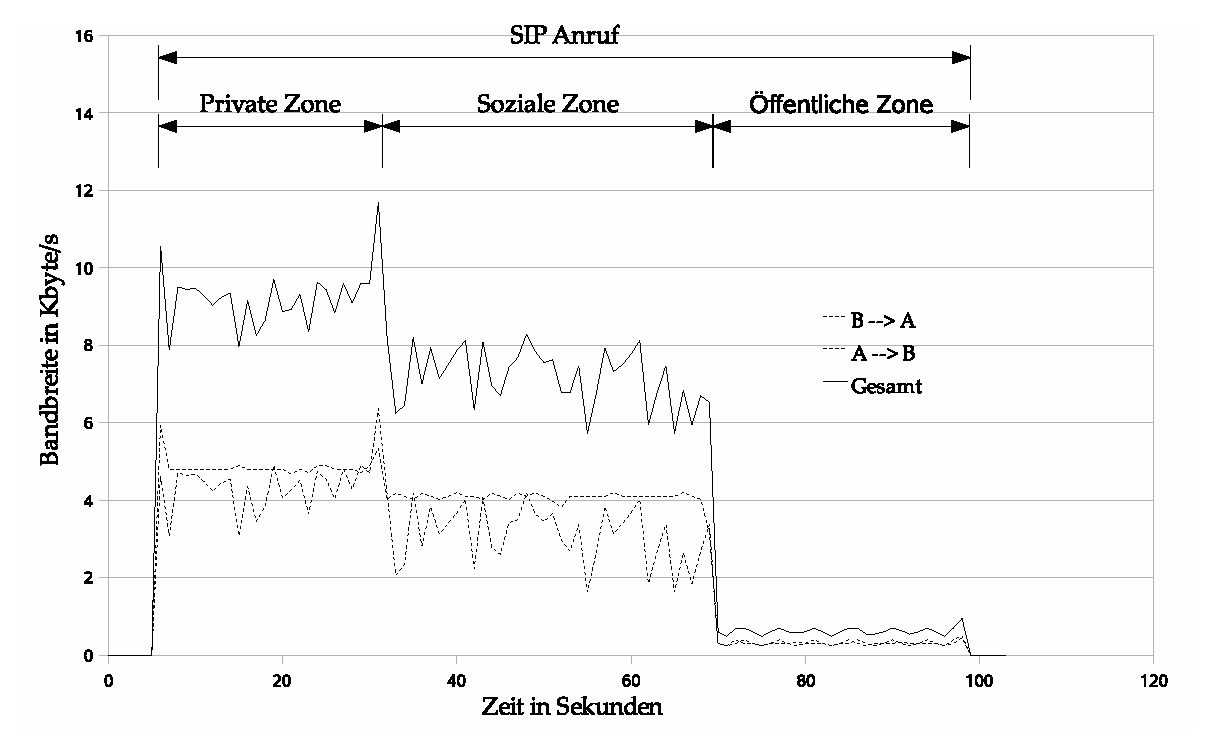
\includegraphics[width=\textwidth]{grafiken/mitvadund2codecs.eps}
		\caption{Speex mit 16 kHz in der privaten Zone und Speex 8 khZ in der sozialen Zone}
	\label{fig:mitvadund2codecs}
\end{figure}

\begin{figure}[tbh]
	\centering
		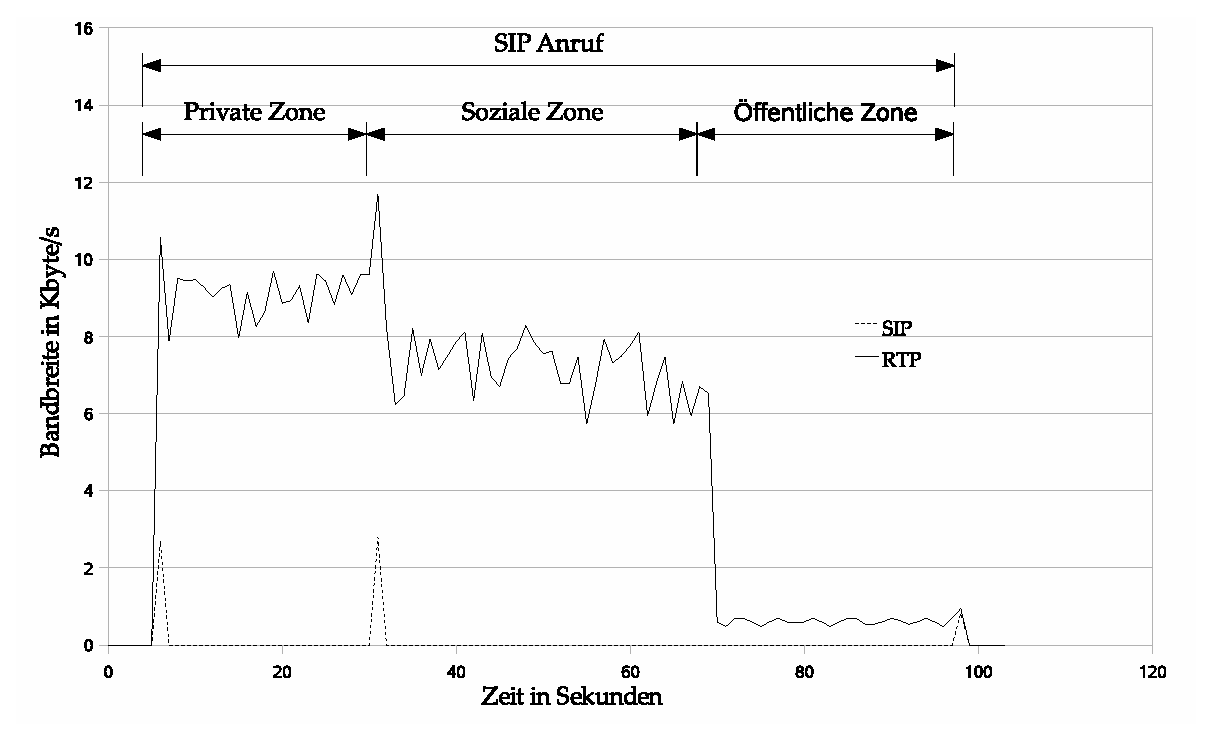
\includegraphics[width=\textwidth]{grafiken/mitvadundrtpsip.eps}
		\caption{Rufauf- und -abbau, sowie Signalisierung eines anderen Codecs mit SIP, Reduktion des Audiostroms mit RTP}
	\label{fig:mitvadundrtpsip}
\end{figure}